\begin{figure}[h]
%\begin{center}
\centering
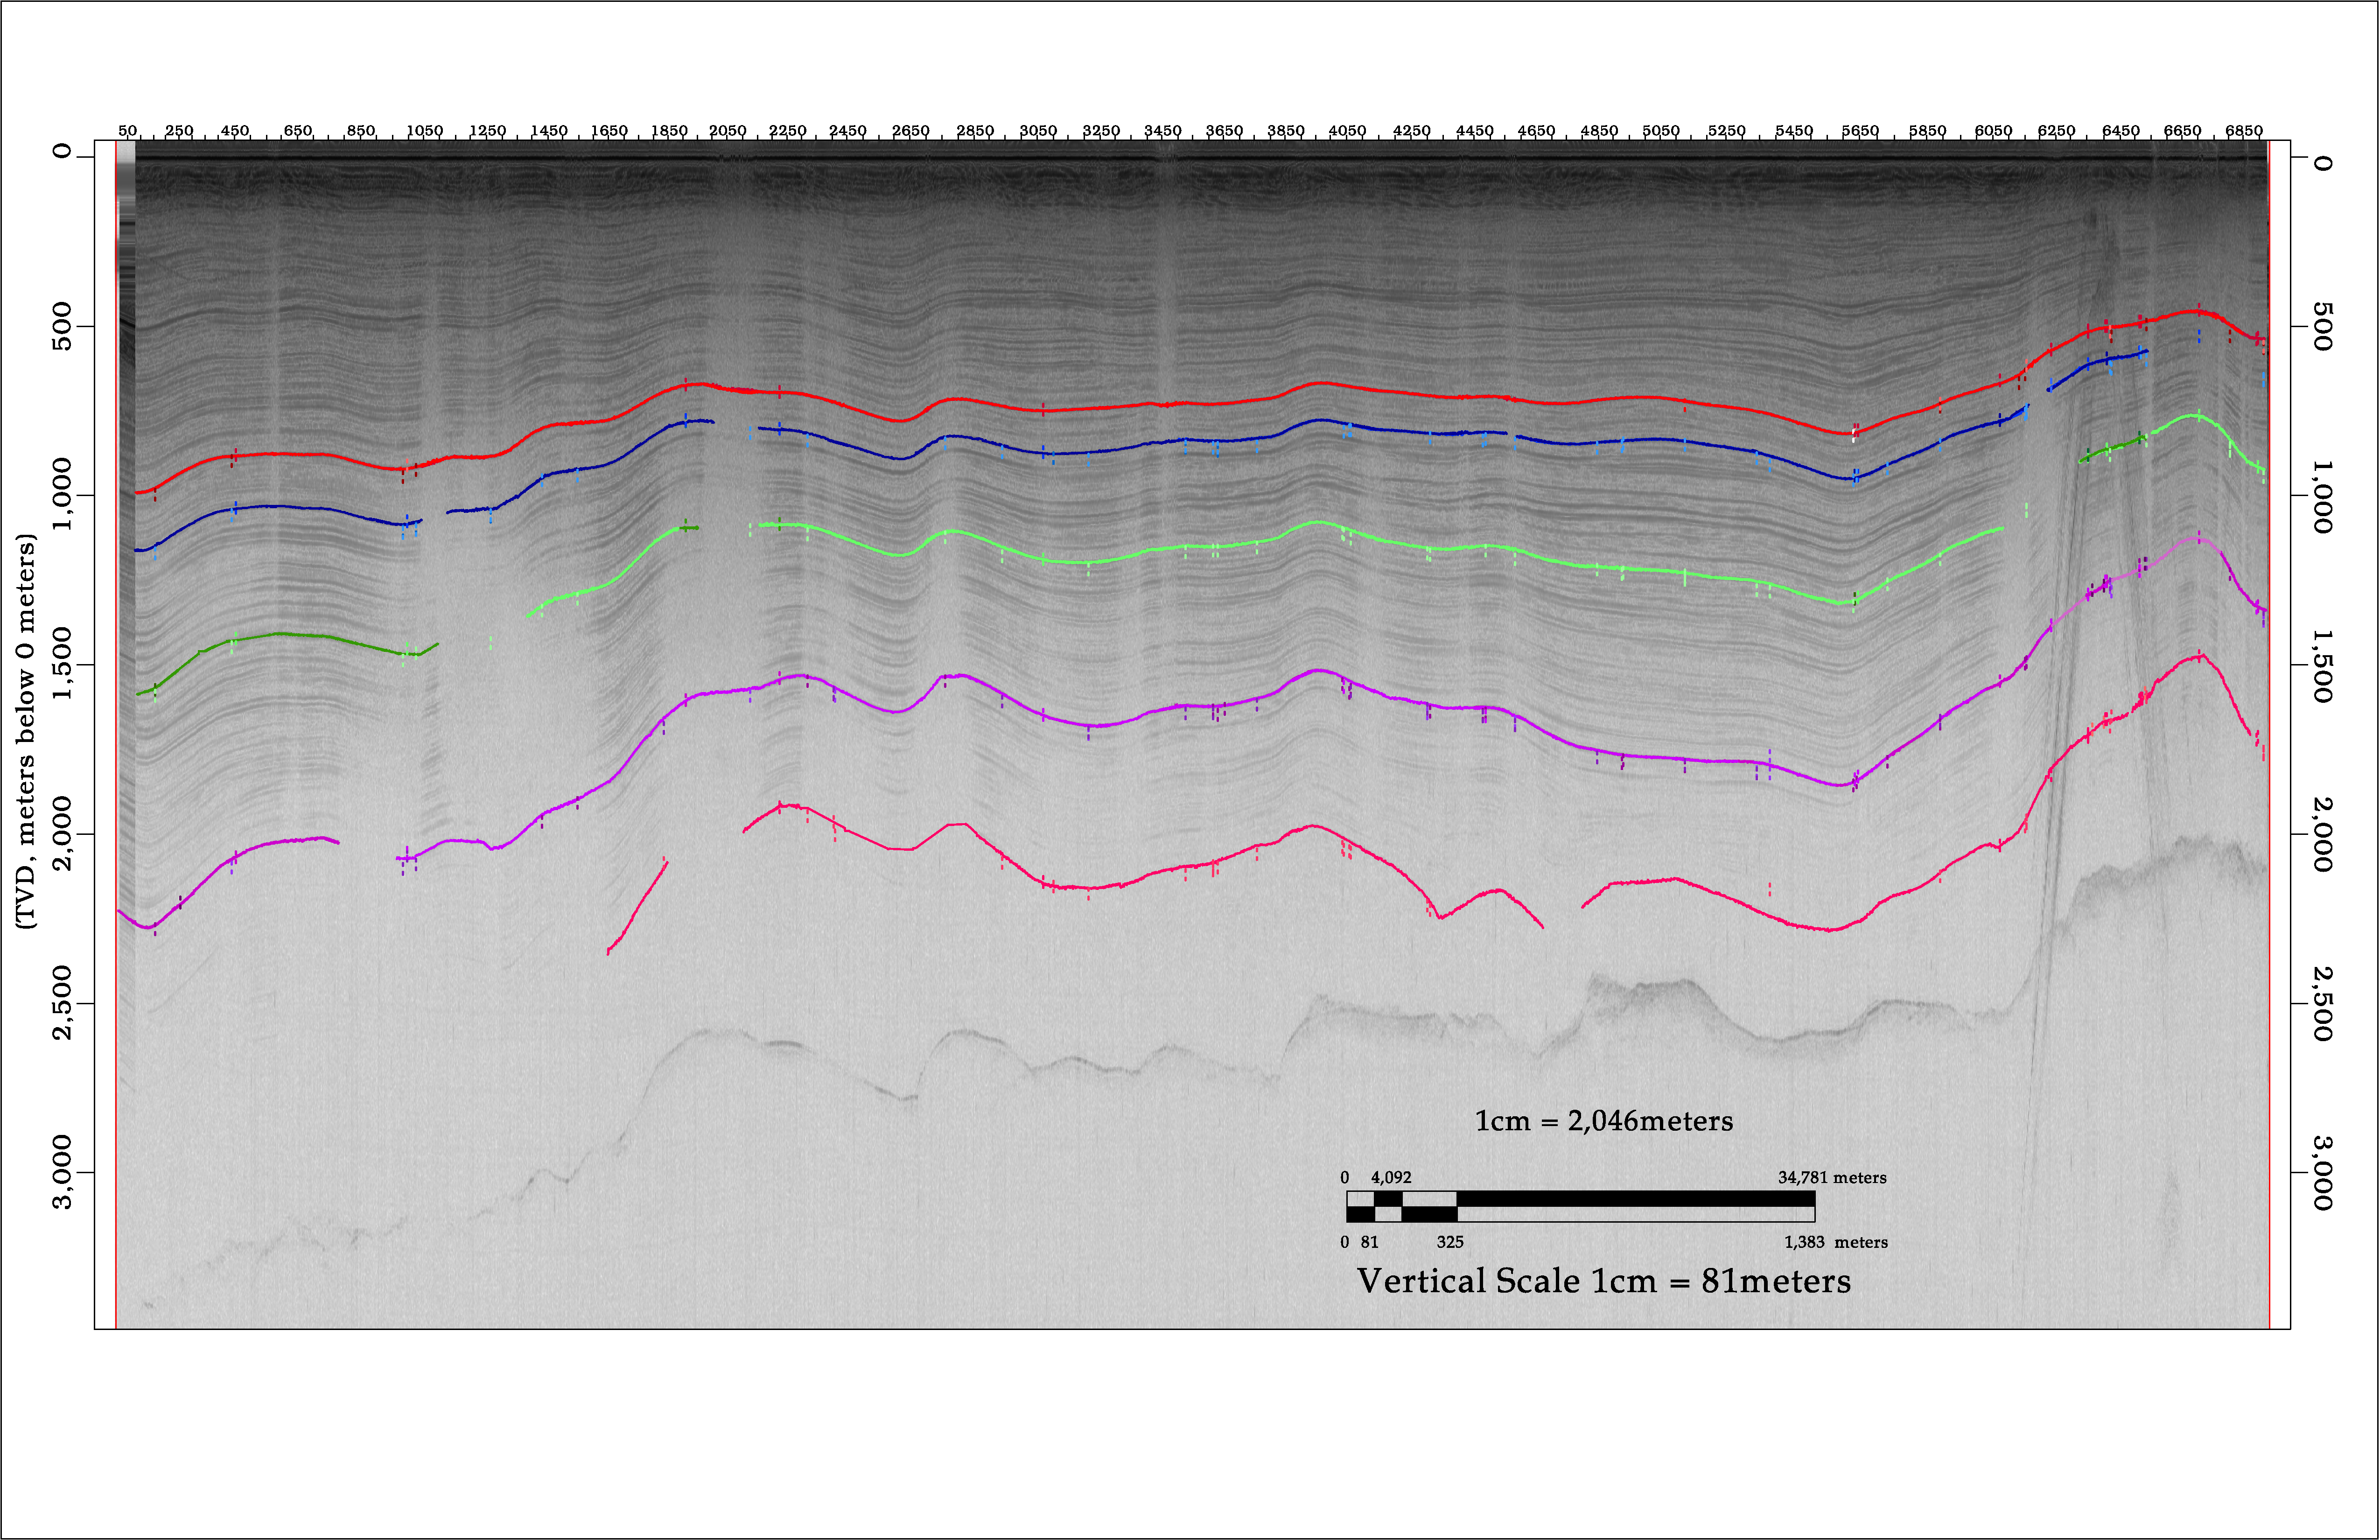
\includegraphics[scale=0.2]{figures/byrd_layers_radargram}
%\captionsetup{width=.9\textwidth}
\caption[]{\textbf{Will be updated to have only four reflectors.} Depth to englacial layers tracked using ice-penetrating radar and Landmark seismic imaging software. Layers shown can be traced between the Byrd and WAIS Divide ice cores. Their ages are shown in Table \ref{tab:depthunc} \textbf{and will be shown on this figure as well in addition to the location of the ice cores}. Relative depth changes between layers can reveal changes in the ice sheet during the interval when they were deposited, as determined by the age of the layers. }
%\end{center}
\label{fig:layergram}
\end{figure}


Radar reflection layers are assumed isochronous, so dating them at one point along their extent makes it possible to know the age of the entire radar layer. Interpolation between flight lines then leads to an isochronous surface within the ice sheet. Due to the extent of radar coverage in central West Antarctica, we have traced 




\begin{figure}[h]
%\begin{center}
\centering
\includegraphics[scale=0.2]{figures/poor-mans-layer-surface-compare}
%\captionsetup{width=.9\textwidth}
\caption[]{\textbf{Obviously not a real figure yet.} Depth to englacial layers tracked using ice-penetrating radar and Landmark seismic imaging software. Layers shown can be traced between the Byrd and WAIS Divide ice cores. Their ages are shown in Table \ref{tab:depthunc} \textbf{and will be shown on this figure as well in addition to the location of the ice cores}. Relative depth changes between layers can reveal changes in the ice sheet during the interval when they were deposited, as determined by the age of the layers. }
%\end{center}
\label{fig:layer_surf}
\end{figure}